\documentclass[11pt]{article}
\usepackage{fullpage,amsmath,amsfonts,mathpazo,microtype,nicefrac,graphicx,verbatimbox,hyperref,listings,enumitem,amssymb,float,fancyhdr}
\hypersetup{
  colorlinks = true
}

\title{
\vspace{1cm}
\textmd{\textbf{AM205 Final Project: Modulo-n Lights Out}}\\
}

\author{\textbf{Shawn Pan and Andrew Ross}}
\date{\today}

%----------------------------------------------------------------------------------------

\begin{document}

\maketitle

\section*{Introduction}

\paragraph{} Lights Out is an electronic puzzle game released by Tiger Electronics (who notably also developed the \href{https://en.wikipedia.org/wiki/Furby}{Furby}) in 1995. An individual puzzle in Lights Out consists of a configuration of lit and unlit buttons on a 5x5 grid. Pressing any button toggles its state and that of the four adjacent buttons, and the goal is to turn all lights off in as few moves as possible.

\paragraph{} The effect of any sequence of presses can be represented as a modulo 2 sum of vectors (where each 2D board coordinate is mapped to a 1D vector position), and because summation is commutative, the sequence of presses will have the same effect regardless of its order. We can represent the constraints of the problem as a system of equations in $\mathbb{Z}_2$ (i.e. modular arithmetic on $\{0, 1\}$), which we can more helpfully write as a matrix equation

\begin{equation}
Ax = b,
\end{equation}

\noindent where $b = \langle g_{11}, g_{12}, \cdots, g_{15}, g_{21}, \cdots, g_{55} \rangle$ is the length-25 vector of grid states $g_{ij}$, which are 1 if lit and 0 otherwise, $x$ is the length-25 vector of presses, and $A$ is a matrix that encodes the transitions. In the standard Lights Out game, $A_{ij}$ is 1 along the main diagonal and, except at 2D board edges, 1 at positions one and five cells above and below the main diagonal. In the more general case, $A$ can be any matrix encoding transitions, the grid can have any dimensions, and transitions can occur not just in $\mathbb{Z}_2$ (modulo 2) but $\mathbb{Z}_k$.

\paragraph{} There are many ways to solve this matrix equation; in the case that $A$ is invertible, we can find its inverse $A^{-1}$ and obtain a unique solution $x = A^{-1}b$. Alternatively, we can use a factorization technique such as the LU decomposition to find $x$ more efficiently. In the case that $A$ isn't invertible, then in general it is possible that there may not be any $x$ such that $Ax = b$, and if there is, then $x$ will no longer be unique (although the shortest $x$, i.e. the $x$ that minimizes $\sum x_i$, may still be).

\paragraph{} \cite{jaap} provides a great analysis of the core mathematics of the game and several variants. In particular, \cite{jaap} devotes a significant amount of time to generalizing board dimensions, with some limited discussion of the game in $\mathbb{Z}_3$, which was released as Lights Out 2000. \cite{giffen} and \cite{involve} approach the problem from the perspective of graph theory and graph coloring problems, generalizing it to arbitrary transition matrices in $\mathbb{Z}_k$. A particular focus of \cite{giffen} and \cite{involve} is determining when the game is always winnable, and on methods of generating families of transition graphs with certain properties.

\paragraph{} Our goal is to reproduce and generalize results from \cite{jaap} and confirm they agree with theorems presented in \cite{giffen} and \cite{involve}. We also want to demonstrate a software package we wrote for solving modular systems of equations and visualizing solutions to Lights Out puzzles.

\paragraph{} Additionally, since solutions to light puzzles (arrays of press patterns) can also be interepreted as grids, we consider the recursive problem of solving a grid, then solving its solution, and so on, until we reach a state we have already seen or one that cannot be solved. The simplest version of this (a complete cycle of length 1) corresponds exactly to eigenvectors of the transition matrix with eigenvalue 1. We will explore these cycles of solutions and attempt to relate them to the theoretical work in \cite{jaap}, \cite{giffen}, and \cite{involve}.

\section*{Nullity and Solvability}

\paragraph{} As we noted above, when $A$ is invertible, then we can solve the puzzle uniquely for any initial board configuration $b$. When $A$ isn't, we are interested in the dimension of its nullspace. In particular, if the nullspace of $A$ is $d$-dimensional, then there will be $d$ linearly independent press patterns that have no effect on the board. These are referred to as "quiet patterns" in \cite{jaap}, and a basis for them can be determined by augmenting $A$ with the identity matrix and performing Gaussian elimination to transform $A$ as close to the identity as possible.

\begin{figure}
\caption{Plots of the dimension of the nullspace of the standard Lights Out transition matrix at various grid sizes and moduli}
\label{nullity}
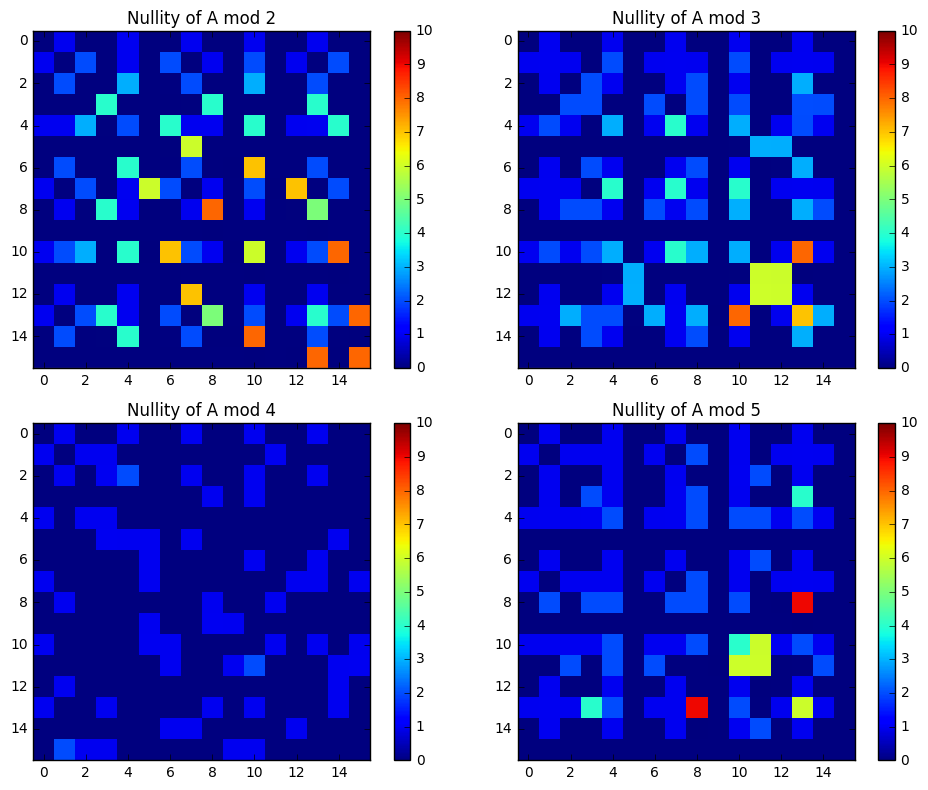
\includegraphics[width=\textwidth]{nullity.png}
\end{figure}

\paragraph{} The dimension of the nullspace can also be determined by performing modulo-$k$ LU factorization on $A$, then counting the number of nonzero entries in the upper-triangular matrix $U$, which is how we calculate it in practice. We do this in Figure \ref{nullity}, which agrees with the tables of results shown in \cite{jaap} for $k=2$ and $k=3$, but generalizes them up to $k=13$.

\begin{figure}
\caption{Plots of theoretical predictions for solvability based on \cite{involve}}
\label{relprime}
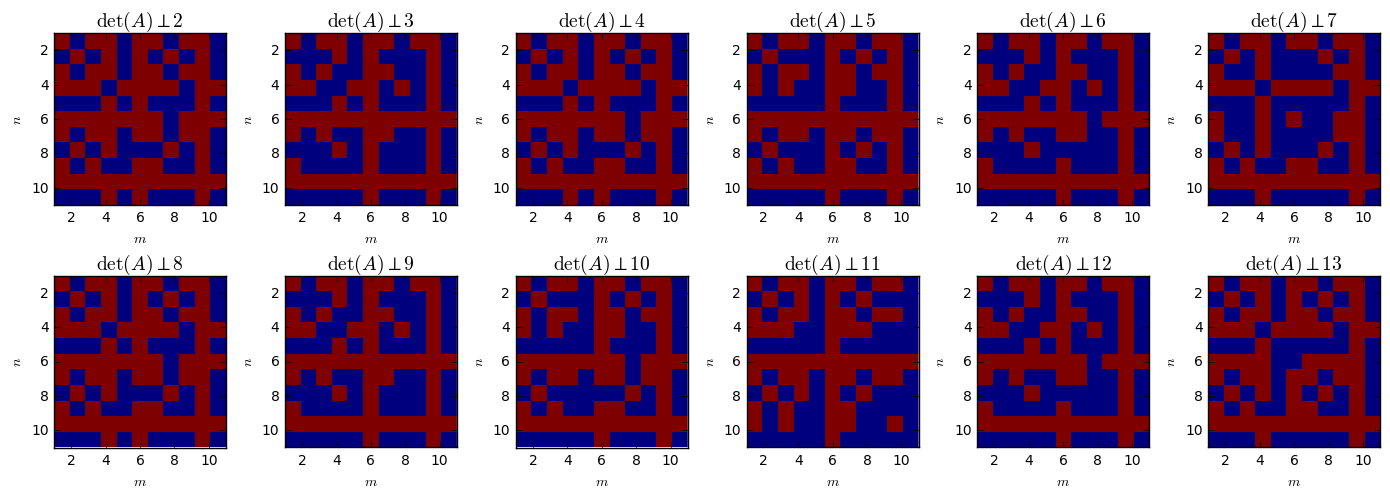
\includegraphics[width=\textwidth]{relprime.png}
\end{figure}

\paragraph{} What's interesting, though, is that our plots in Figure \ref{nullity} actually disagree in certain cases with a theoretical result from \cite{involve}, which states that $A$ must span $\mathbb{Z}_k$ if $det(A)$ and $k$ are coprime (i.e. their greatest common denominator is 1). Figure \ref{relprime} shows plot of those theoretical predictions, which you can see agree with the results in Figure \ref{nullity} but only when $k$ is prime. Coincidentally, \cite{involve} only proves that result for prime values of $k$, but it is unclear whether their result actually doesn't hold for non-prime values of $k$ (or if there is an error in our code).


\section*{Solving Matrices in a Modular Field}


\section*{Singular Transition Matrices}
\paragraph{} Although LU factorization followed by forward and backward substitution works well for solving full rank matrices, the default procedure does not work for singular matrices.  When exploring the light out problem, we often run into this issue.  For example, consider the transition matrix for the standard 5x5 lights out game.  The matrix has rank 23 and nullity 2.  The interpretation is that not all states in the game are reachable from a blank grid.  The game has a solution space of $2^{23}$ states and null space of $2^2$ states.


\paragraph{} We have adapted the algorithm to deal with the singular cases.  The rank of the matrix is equal to the number of non-zero entries along the upper diagonal factor $U$.  Therefore, we may proceed as usual with the standard algorithm until the backward substitution step.  In the backward substitution step, we will run into $n$ zero diagonal entries, where $n$ is the nullity of the original matrix.  These zero diagonal entries correspond to equations of the form $0 = 0$ or $0 = 1$.  In the $0 = 1$ case, the system is inconsistent and has no solutions.  In the $0 = 0$, the system has multiple solutions, because we essentially have an unconstrained free parameter.


\paragraph{} Consider a particular zero diagonal entry $U_{ii} = 0$.  We can change the matrix to be no longer singular by setting $U_{ii} = 1$, essentially adding an extra equation to the system.  We do not have any constraint on $x_i$ and can set it to any of value from 0 to $m - 1$ for a field with modulus $m$.  We consider 3 different ways to picking the free parameter $x_i$, and our solve method takes in a flag for which method to use.

\begin{itemize}
\item Any: We pick all $x_i$ to be 0, which will return an arbitrary solution.
\item Basis: For each of the $n$ zero diagonal entries, we perform a reverse solve with only that $x_i$ set to 1 and all other free parameters set to 0.  This procedure finds $n$ solutions which form a basis for the nullspace.
\item All: For each of the $m^n$ possible free parameter choices for $x_i$, we perform a reverse solve.  This procedure finds all possible solutions to the equation.  The number of solutions grows exponentially with the dimensions of the nullspace.
\end{itemize}

\subsection*{Applications}
finding eigenvalues and quiet states



\section*{Eigengrids and Solution Cycles}

\paragraph{} Eigengrids (with eigenvalue 1) are characterized by the following equation:

\begin{equation}
Ax = x,
\end{equation}

\noindent and repeating solution "cycles" (of period $n$) are characterized by:

\begin{equation}
A^nx = x,
\end{equation}

\noindent or in other words, $x$ is an eigengrid of $A^n$. For certain dimensions, modulos, and transition functions, we found that $A^n$ commonly tended to equal the identity matrix for some $n$. We also found cases where

\begin{equation}
\begin{split}
  A^{n_1 + n_2}x & = A^{n_1}x,\\
  A^{n}x & \neq x \text{ for all } n,
\end{split}
\end{equation}

\noindent that is, where after $n_1$ "iterations" of solving solutions, we would enter a repeating solution cycle with period $n_2$ that didn't contain our initial set of $n_1$ transient states.

\paragraph{} Let us consider the example of our normal Lights Out transition matrix $A \% 6$ on a 2x2 grid. We choose this example in part because there are a manageable but large number of possible grids ($6^{2 \times 2} = 1296$), and in part because our calculated nullity for this matrix disagrees with the predictions of \cite{involve}. We will iterate through each of the 1296 possible button grids $b$, solve $Ax=b$, and repeatedly re-solve our solutions until we reach a steady state.

\paragraph{} First, we find that we appear to be able to solve $Ax=b$ for every $b$, despite the fact that $\det(A) = -3$ is not coprime to $k=6$. Second, we find that for this case (unlike the set of solutions at lower values of $k$, which we also calculated), there are many transient states, that, when repeatedly solved, lead to a cycle that does not contain them.



\begin{figure}
\caption{The twelve eigenstates of $A_{\% 6}$ on a 2x2 grid}
\label{eig622}
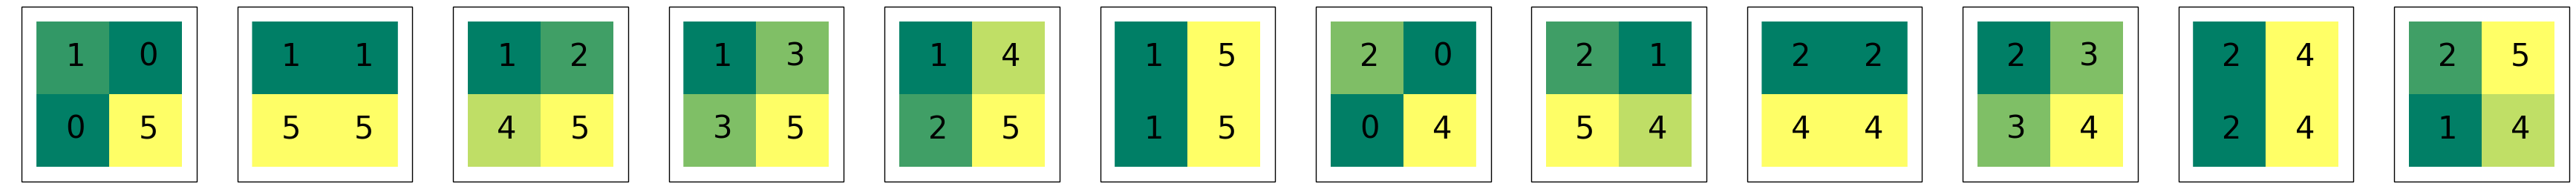
\includegraphics[width=\textwidth]{eig622.png}
\end{figure}

\begin{figure}
  \caption{A 3-state transient path ending in a 6-state cycle of $A_{\% 6}$ on a 2x2 grid}
\label{cycle622}
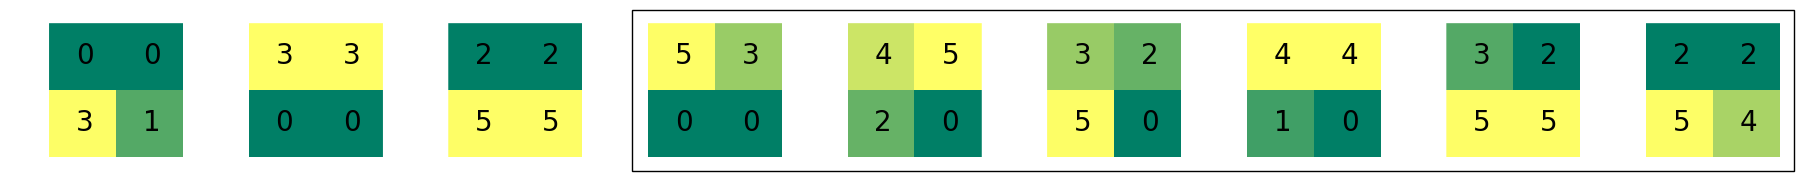
\includegraphics[width=\textwidth]{cycle622.png}
\end{figure}

\begin{figure}
\caption{The twelve 6-state cycles of $A_{\% 6}$ on a 2x2 grid}
\label{cycle622}
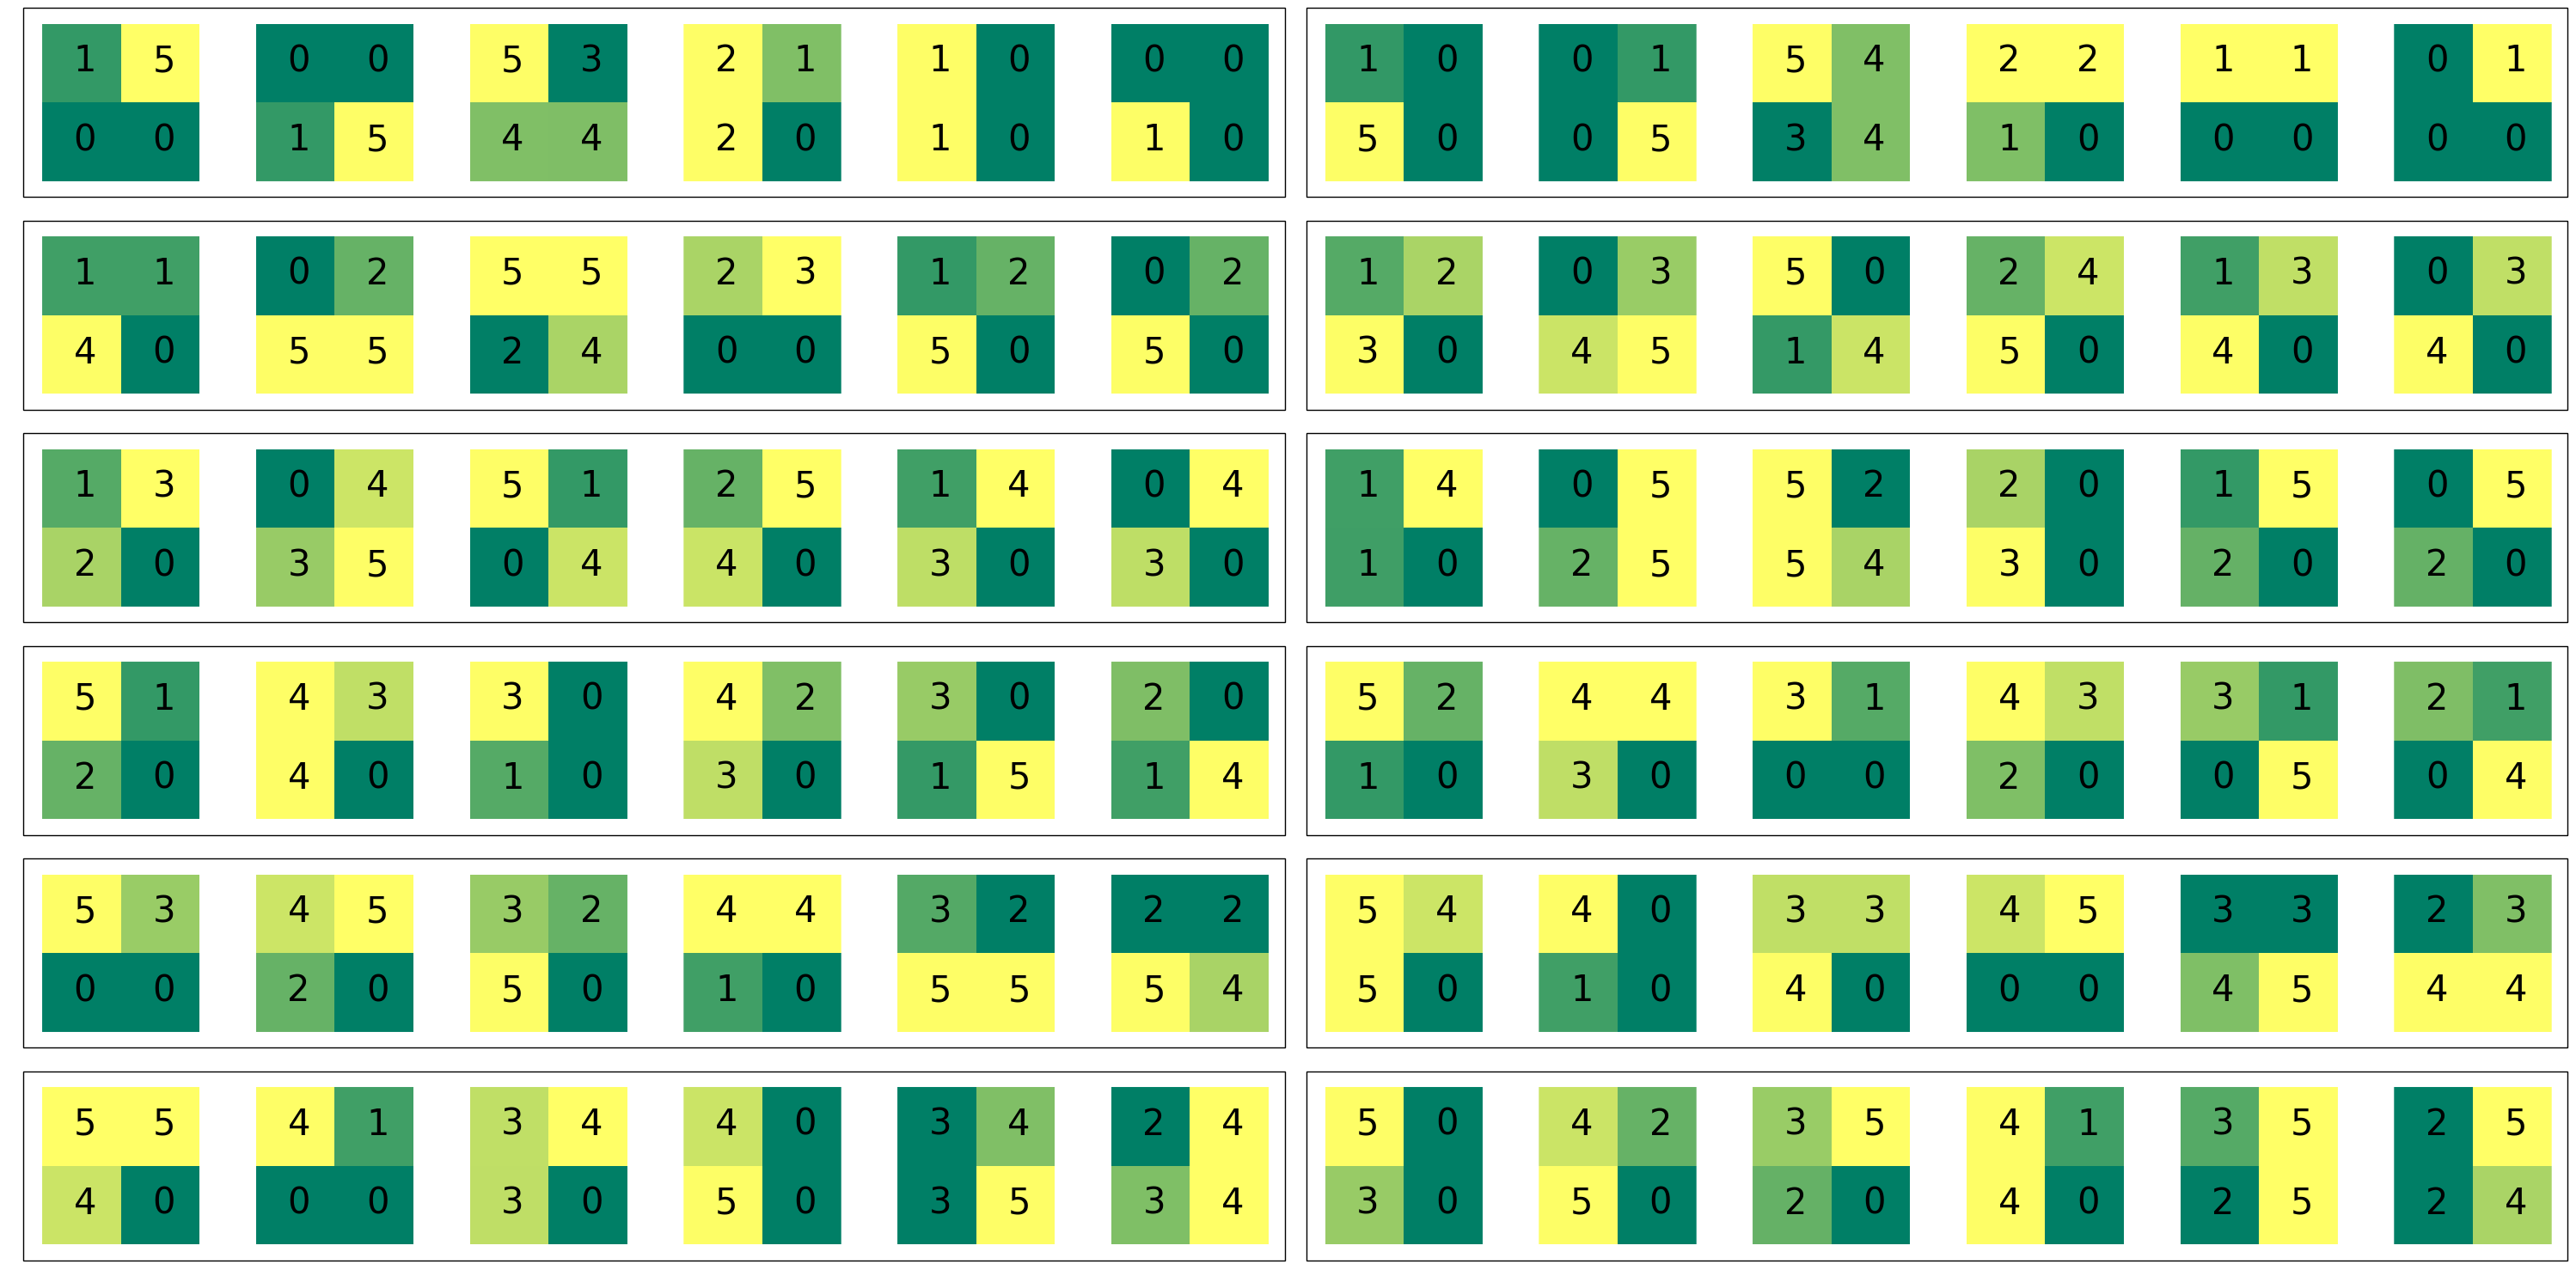
\includegraphics[width=\textwidth]{all-len-6-cycles-622.png}
\end{figure}

\begin{tabular}{|l|l|l|l|l|l|}
  \hline
  & \multicolumn{5}{|c|}{Sq. Grid Length} \\ \hline
  $k$ & \textbf{1} & \textbf{2} & \textbf{3} & \textbf{4} & \textbf{5} \\ \hline
  \textbf{2} & 2 & 4 & 8 & $\emptyset$ & $\emptyset$ \\ \hline
  \textbf{3} & 3 & $\emptyset$ & 27 & $\emptyset$ & $\emptyset$ \\ \hline
  \textbf{4} & 4 & 16 & \\ \hline
  \textbf{5} & 5 & 25 \\ \hline
\end{tabular}


\section*{Visually Appealing Solutions}

\clearpage

\begin{thebibliography}{9}
\bibitem{jaap}
  J. Scherphuis, \textit{The Mathematics of Lights Out},
  \href{http://www.jaapsch.net/puzzles/lomath.htm}{http://www.jaapsch.net/puzzles/lomath.htm}.
  Accessed December 2016.
\bibitem{giffen}
  A. Giffen and D. B. Parker, \textit{On Generalizing the "Lights Out" Game and a Generalization of Parity Domination}, preprint, 2009. Available at \href{http://faculty.gvsu.edu/parkerda/profstuff/papers/hyperlogpd.pdf}{http://faculty.gvsu.edu/parkerda/profstuff/papers/hyperlogpd.pdflink}.
\bibitem{involve}
  S. Edwards, V. Elandt, N. James, K. Johnson, Z. Mitchell, and D. Stephenson, \textit{Lights Out on finite graphs}, Involve 3 (2010), 17-32. Available at \href{http://msp.org/involve/2010/3-1/involve-v3-n1-p03-s.pdf}{http://msp.org/involve/2010/3-1/involve-v3-n1-p03-s.pdf}.
\end{thebibliography}

\end{document}
